% informe.tex - Documentación sobre el trabajo práctico para entregar

\documentclass{article}
\usepackage[utf8]{inputenc}
\usepackage[spanish]{babel}
\usepackage{graphicx}

\begin{document}

\title{Informe Trabajo Práctico 1 - Técnicas de Programación Concurrente (75.59)}
\author{Victoria Perelló (89608)\\
        \and
        Agustín Mezzina (89637)\\
	\and
        Pablo Rodríguez (93970)}
\maketitle

\tableofcontents
\clearpage

\section{Introducción}
\subsection{Descripción del problema}
El presente trabajo práctico consiste en una simulación de la dinámica de operación de una estación de servicio. En ella, los operarios deben atender a los clientes entrantes utilizando los recursos de los cuales dispone la estacion. El eje del problema es la comunicación y la sincronización de los operarios en el uso de dichos recursos para el correcto funcionamiento del negocio.
\subsection{Modo de uso}
Adjunto a este informe se encuentra el código fuente de la aplicación y un archivo Makefile para realizar la compilación. El sistema debe ser compilado utilizando la directiva ``make all'', el cuál generará cinco ejecutables con los programas que van a interactuar en el sistema.
Para comenzar la simulación, debe ejecutarse en una consola el archivo ``ConcuStation''.
El sistema pedirá al usuario que ingrese el número de empleados y de surtidores que posee la estación. Luego de ingresados, dará inicio a la simulación.
Durante el transcurso de la misma, el usuario puede ingresar dos comandos por entrada estándar:
\begin{enumerate}
	\item ``c'': Consultar Caja. Imprime por salida estándar la recaudación actual de la Caja.
	\item ``q'': Finalizar simulación.
\end{enumerate}


\section{Procesos}
La aplicación se divide en los siguientes procesos:
\begin{enumerate}
	\item Init: genera un auto cada cierta cantidad aleatoria de tiempo transcurrido y los envía al jefe de estación para su procesamiento.
	\item Jefe de estación: recibe los autos entrantes y los asigna a empleados libres. En caso de no haber empleados libres, los despacha.
	\item Empleado: asigna autos a surtidores libres. Si no hay surtidores libres, espera a que se libere alguno. Realiza el servicio. Cobra y guarda la recaudación en la caja.
	\item Consulta caja registradora: consulta asincrónica sobre el valor de la recaudación en caja.
	\item Lector de comandos: escucha comandos entrantes por entrada estándar y toma las medidas correspondientes para responder a ellos.
\end{enumerate}

\section{Comunicación entre procesos}
En el siguiente diagrama, se muestra el esquema de comunicación entre los procesos del sistema. Incluye los datos que intercambian los procesos que se comunican entre sí y los recursos a los que deben acceder de manera concurrente.
\\[1\baselineskip]
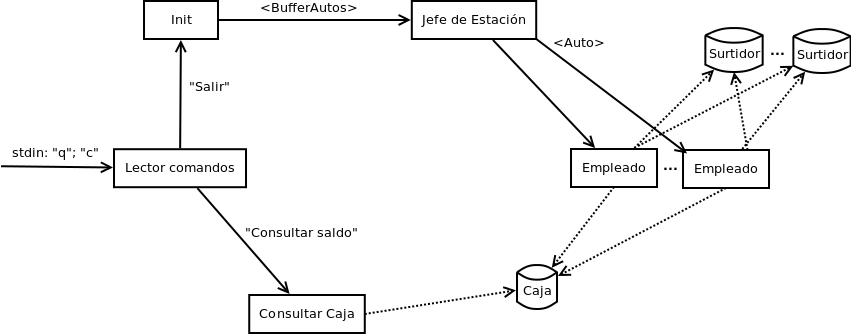
\includegraphics[width=\textwidth]{overview}

\section{Problemas típicos de concurrencia}
\begin{enumerate}
	\item Init - Jefe de estación: Productor - Consumidor. El proceso base hace las veces de Productor, ingresando autos nuevos a un buffer compartido donde posteriormente el Jefe de Estación, en este caso Consumidor, los retira según su orden de llegada y los procesa.
	\item Jefe de estación - Empleado(s): Productor - Consumidor. Se presenta un caso similar al anterior, con la variante de que el Productor (Jefe de estación) debe determinar a cuál de los Consumidores (Empleados) enviar el recurso generado.
	\item Empleado - Empleado: Sección Crítica. Los procesos deben excluirse mutuamente al ejecutar código que acceda a los recursos Surtidores, ya que el mismo Surtidor no puede ser utilizado por dos Empleados al mismo tiempo.
	\item Empleado(s) - Consultar Caja: Sección Crítica. Los procesos deben excluirse mutuamente al acceder a la Caja, ya sea para leer como para escribir.
\end{enumerate}
\section{Mecanismos de concurrencia a utilizar}
En el siguiente diagrama se muestran los mecanismos de concurrencia utilizados para lograr la comunicación y sincronización de procesos:
\\[1\baselineskip]
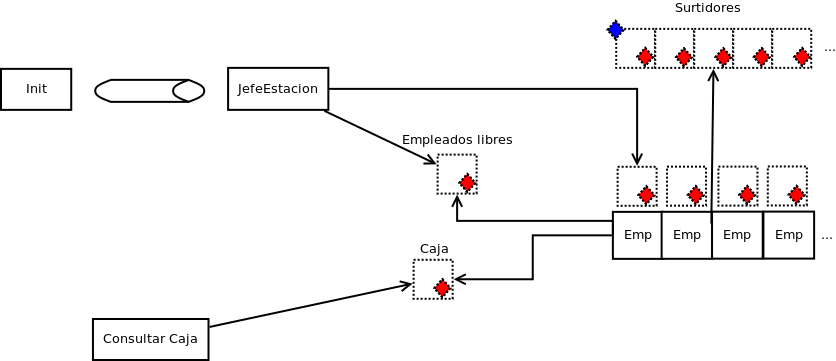
\includegraphics[width=\textwidth]{mecanismos}
\subsection{Init - Jefe de estación}
El buffer de autos se implementó utilizando un named pipe (o FIFO), de manera que el proceso inicial ingresa los autos al canal a medida que los va produciendo y el jefe de estación los toma en orden para procesarlos. Este mecanismo de concurrencia provee no sólo comunicación entre ambos procesos, sino que también sincronismo.
\subsection{Jefe de estación - Empleado(s)}
Cada Empleado mantiene con el Jefe de Estación un espacio de intercambio en memoria compartida, donde se guarda información sobre el estado del Empleado (libre u ocupado) y el auto que debe ser atendido. Cada uno de estos espacios de intercambio está protegido con un semáforo binario para lograr exclusión mutua entre el Jefe y el Empleado correspondiente en el acceso al mismo, ya sea para lectura o para escritura.
\subsection{Empleado - Empleado}
Los Surtidores están guardados en bloques de memoria compartida accesibles a todos los Empleados. Dicho bloque está protegido por un semáforo general que permite el acceso al área de memoria cuando haya algún surtidor libre. Cada espacio de memoria donde se encuentra un surtidor está, a su vez, protegido por un semáforo binario.
\subsection{Empleado(s) - Consultar Caja}
Estos procesos acceden a un espacio de memoria compartida donde está la Caja. Se excluyen mutuamente mediante un semáforo binario para coordinar el acceso a la misma.

\section{Otras consideraciones}
\subsection{Inicio y finalización}
Al iniciar la simulación, el proceso Init crea todas las memorias compartidas y semáforos (estos últimos también los inicializa) necesarios para el funcionamiento del sistema, así como también el FIFO que sirve como canal de comunicación con el Jefe de empleados. Luego lanza los procesos Jefe de Empleados, Lector de Comandos y todos los Empleados. El proceso Consultar Caja es lanzado por el Lector de Comandos cada vez que el usuario ingresa el comando ``c''. Este proceso finaliza luego de imprimir el valor de la Caja en pantalla.
Cuando el Lector de Comandos recibe el comando ``q'', el sistema debe finalizar. Para esto, se envía la señal SIGTERM al proceso Init y este, a su vez, envía una señal similar a todos los Empleados y un mensaje especial al Jefe de Estación a través del FIFO. Estos procesos manejarán los mensajes eliminando todos sus recursos y finalizando correctamente. El proceso Init espera la finalización de los demás procesos y luego procede a elminar todos los canales de comunicación creados inicialmente, para luego finalizar.
\subsection{Log}
Todos los procesos de la simulación informan las acciones que realizan mediante la escritura a un único archivo denominado ``ConcuStation.log''. El mismo puede utilizarse para verificar el funcionamiento del sistema y el orden en el que se realizan las actividades. Para coordinar el acceso al archivo, se utilizan locks de escritura.

\section{Diagramas}
\subsection{Diagrama de clases}
Mecanismos de concurrencia:
\\[1\baselineskip]
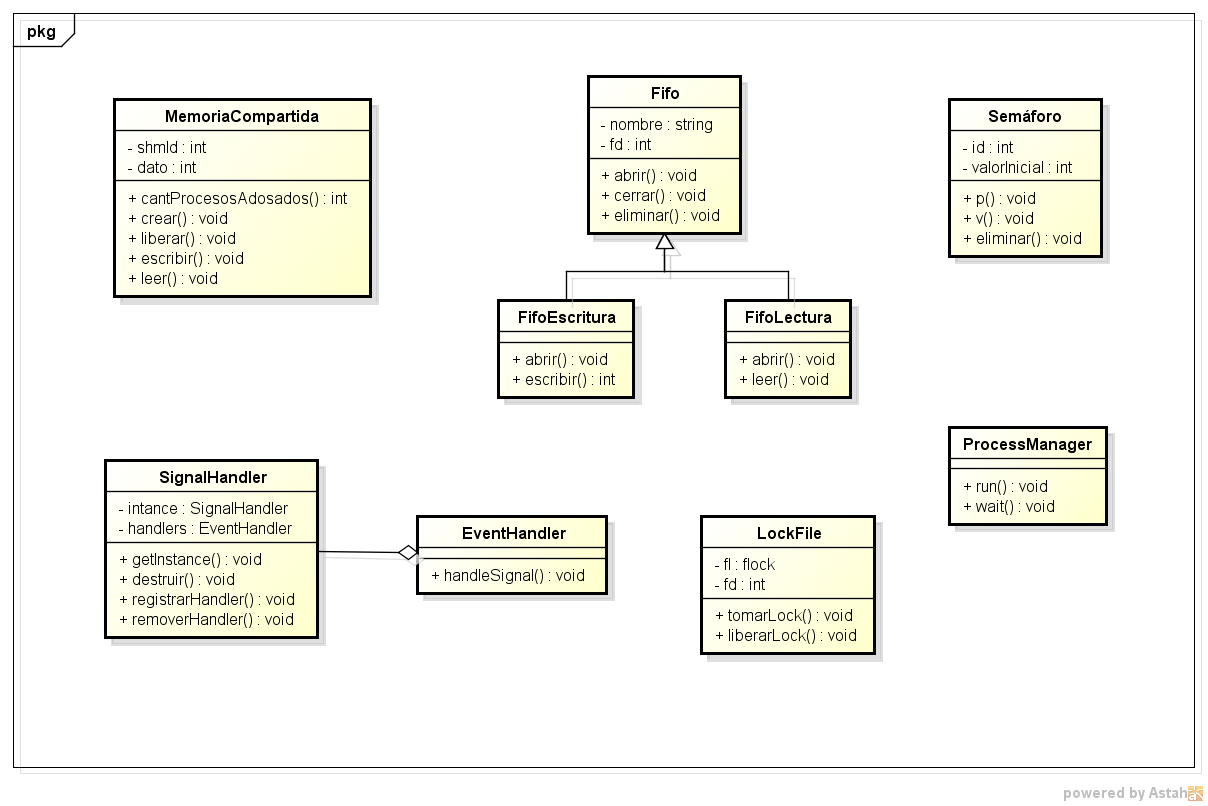
\includegraphics[width=\textwidth]{clasesConcurrencia1}
Recursos:
\\[1\baselineskip]
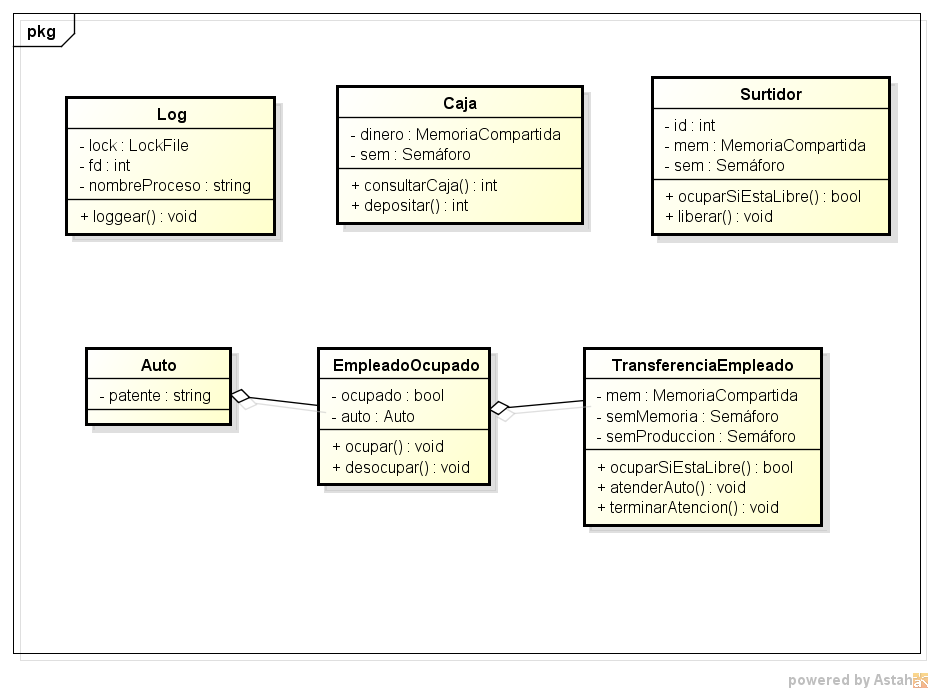
\includegraphics[width=\textwidth]{clasesConcurrencia2}
Procesos:
\\[1\baselineskip]
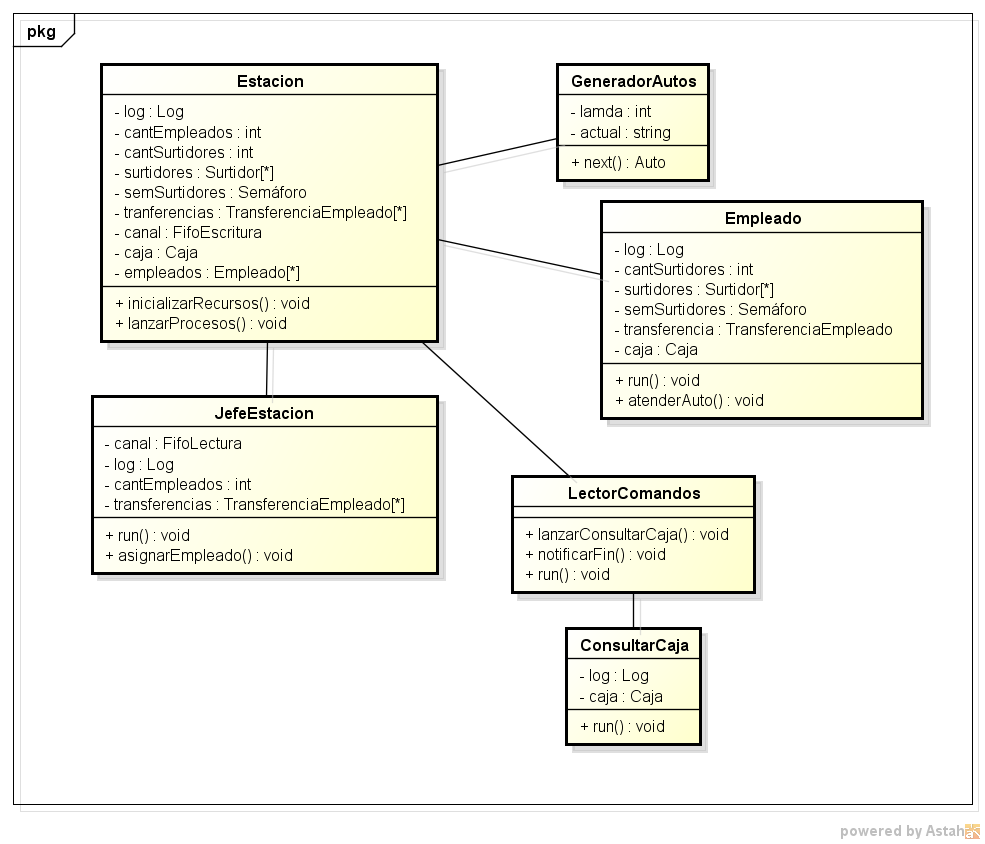
\includegraphics[width=\textwidth]{clasesConcurrencia3}
\subsection{Diagrama de transición de estados: Jefe de Estación}
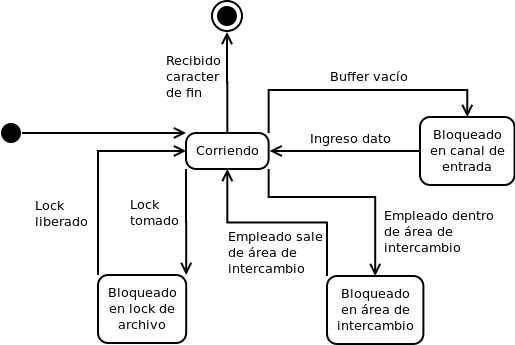
\includegraphics[width=\textwidth]{diagramaTransicionEstadosJefe}
\end{document}
